\documentclass[12pt, a4paper]{book}
\usepackage[a4paper, total={6in, 8in}]{geometry}
\usepackage[english]{babel}
\usepackage{ragged2e}
\usepackage{ragged2e}
\usepackage{fancyhdr}
\usepackage{lastpage}
\usepackage{graphicx}
\usepackage{hyperref}
\graphicspath{{images/}}

\def\thesection{\Roman{section}}
\def\thesubsection{\Roman{section}.\Roman{subsection}}
\def\thesubsubsection{\Roman{section}.\Roman{subsection}.\Roman{subsubsection}}

\pagenumbering{arabic}

\pagestyle{fancy}
\fancyhf{}

\lfoot{{\small Rev. 1.0}}
\rfoot{{\small Page \thepage \hspace{1pt} of \pageref{LastPage}}}

\title{\textbf{{\LARGE G.A.I.A.} \\ User Manual \\ {\small v1.0.0} }}
\author{T\&L}
\date{September 2022}

\setcounter{secnumdepth}{0} % sections are level 1

% MACROS
\newcommand*{\thead}[1]{\multicolumn{1}{|c|}{\bfseries #1}}

\begin{document}
\maketitle

\addtocontents{toc}{\protect\setcounter{tocdepth}{-1}}
% From this point on, only show up to \chapters in the ToC
\newpage
\section {Abstract}

\begin{justify}
This user manual describe how to use G.A.I.A. and more in details how to control the behaviour using configuration file.
\end{justify}


\addtocontents{toc}{\protect\setcounter{tocdepth}{3}}
% From this point on, only show up to \subsection in the ToC

% Table of Contents
\tableofcontents

\addtocontents{toc}{\protect\setcounter{tocdepth}{-1}}
% From this point on, only show up to \chapters in the ToC

\newpage
\begin{center}
\textbf{{\large Document Management}}
\end{center}

\begin{table}[h]
\centering
	\begin{tabular}{|l|l|c|}
	\hline
	Author & T\&L & 16/09/2022 \\
	\hline	
	Issued by & & \\
	\hline
	Revised by & & \\
	\hline
	Approved by & & \\
	\hline
	\end{tabular}	 	
\end{table}

\begin{center}
\textbf{{\large Document Status Sheet}}
\end{center}

\begin{table}[h]
\centering
	\begin{tabular}{|c|c|l|}
	\hline
	\thead{ Issue } & \thead{ Date } & \thead{ Comment } \\
	\hline	
	1.0 & 23/09/2022 & First Release \\
	\hline
	& & \\
	\hline
	& & \\
	\hline
	\end{tabular}	 	
\end{table}

\begin{center}
\textbf{{\large Document Change Record}}
\end{center}


\begin{table}[h]
\centering
	\begin{tabular}{|l|l|c|c|}
	\hline
	\thead{ Issue } & \thead{ Reason for change } & \thead{ Paragraph } & \thead{ Type of Modification } \\
	\hline	
	& & & \\
	\hline
	& & & \\
	\hline
	& & & \\
	\hline
	\end{tabular}	 	
\end{table}



\addtocontents{toc}{\protect\setcounter{tocdepth}{3}}
% From this point on, only show up to \subsection in the ToC

\newpage
\section{Introduction}

The GTFS is largely used for 

\subsection{Purpose}
\subsection{Scope}

\subsection{Definitions}
\subsection{Abbreviations}
\subsection{Reference Documents}
{\small [1] \url{https://developers.google.com/transit/gtfs}}

\newpage
\subsection{Document Overview}

\begin{justify}
This manual is intended for GAIA users that would like to customise their.
\end{justify}

%\justifying


\begin{figure}[h]
    \centering
    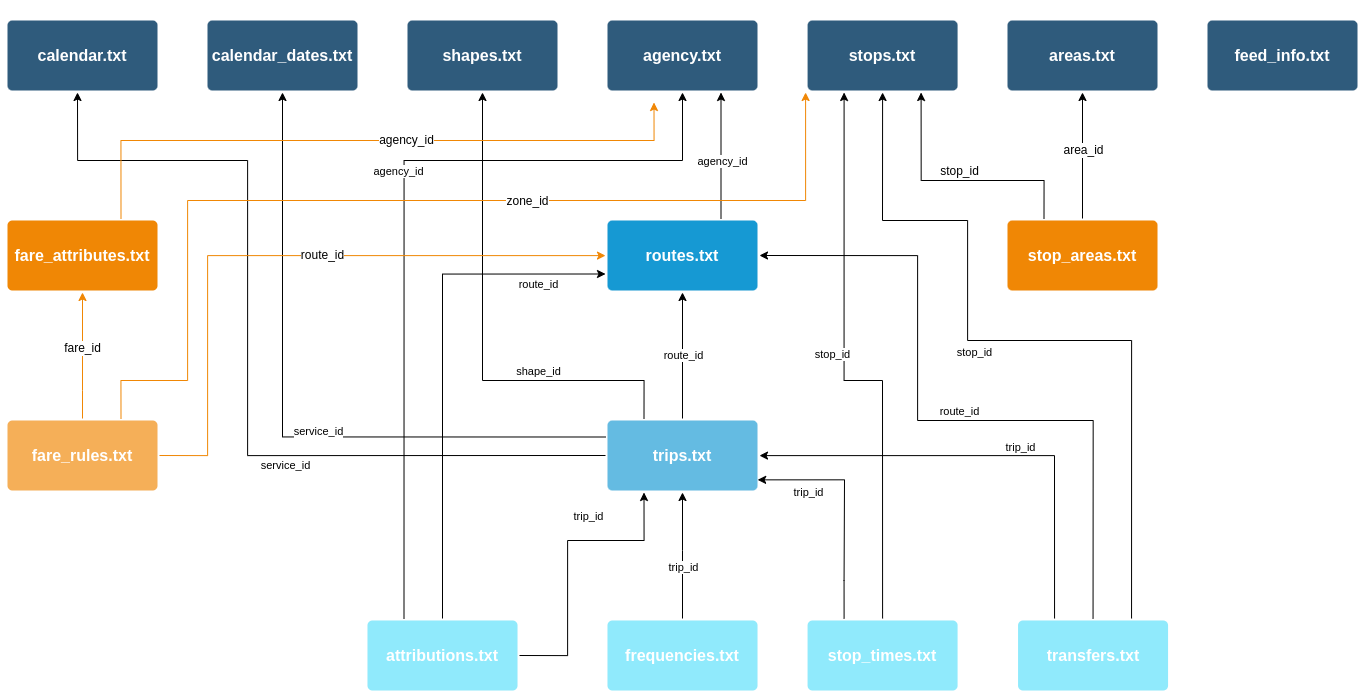
\includegraphics[width=1.0\textwidth]{GTFS Diagram}
    \caption{GTFS Dependencies}
    \label{fig:figure1}
\end{figure}

%\section{First Example}


\end{document}

